% \bibliography{../src/bibliography}

In this chapter I give the nescessary background

\section{Syntax}
\begin{itemize}
  \item Some generic stuff on syntax and constituency in natural language
  \item Reference \citep{Carnie2010:constituent,Everaert+2015:structures} or something?
\end{itemize}

\section{Parsing}
\begin{itemize}
  \item Treebanks, in particular the Penn Treebank. Treebank preprocessing. CFGs, CNF, spans. Reference figure \ref{fig:trees}.
  \item The two conceptions of a tree: as a set of \textit{labeled spans} or as a set of \textit{anchored rules}.
  \item A labeled span is a triple $(\ell, i, j)$ of a syntactic label $\ell$ together the left and right endpoints $i$, $j$ that the label spans.
  \item An \textit{anchored rule} is a four-tuple $(r, i, k, j)$ containing the CNF rule $r$ with the span endpoints $i$, $j$ and split-point $k$ of the left and right child (TODO: unary rules)
  \item For the difference, consider the following two representations of the tree in figure \ref{fig:tree-cnf-spans} given in table \ref{tab:spans-rules}.
  \item Algorithms for parsing: global chart based, local transition based
  \item Dynamic programming inference versus search heuristics.
  \item Modelling types: generative, discriminative, log-linear, count-based, feature-based, neural network features.
\end{itemize}

\begin{figure}
	\centering
  \begin{subfigure}{0.72\textwidth}
		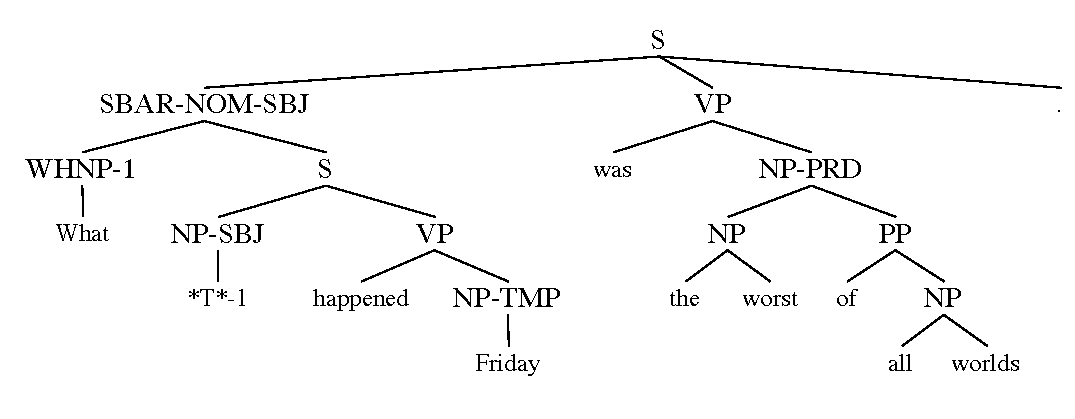
\includegraphics[width=\textwidth]{../figures/trees/original.pdf}
    \caption{Original Penn Treebank tree.}
		\label{fig:tree-original}
	\end{subfigure}
	\begin{subfigure}{0.62\textwidth}
		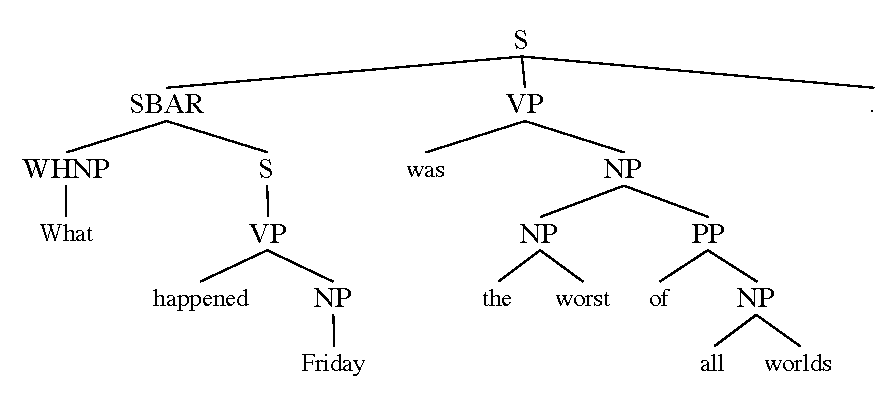
\includegraphics[width=\textwidth]{../figures/trees/simplified.pdf}
    \caption{Function tags and traces removed.}
		\label{fig:tree-simplified}
	\end{subfigure}
	\begin{subfigure}{0.62\textwidth}
		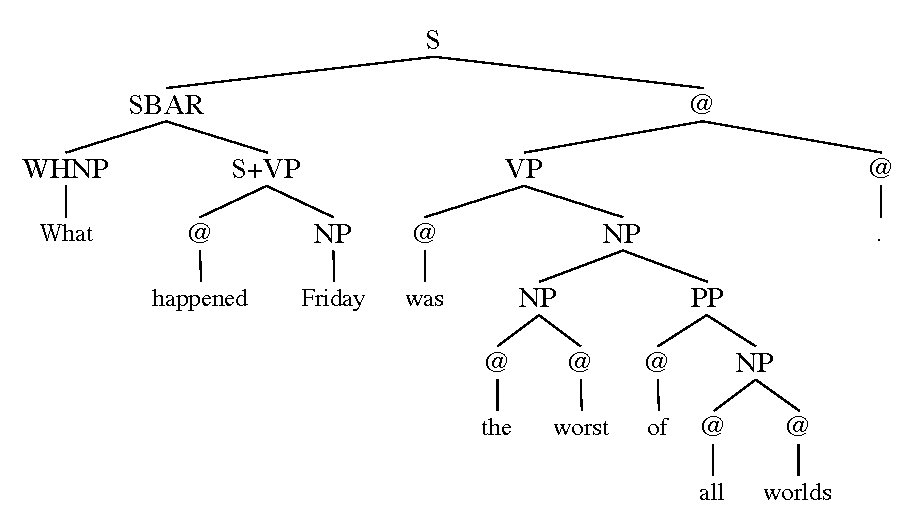
\includegraphics[width=\textwidth]{../figures/trees/binary.pdf}
    \caption{Converted to normal form.}
		\label{fig:tree-cnf}
	\end{subfigure}
	\begin{subfigure}{\textwidth}
		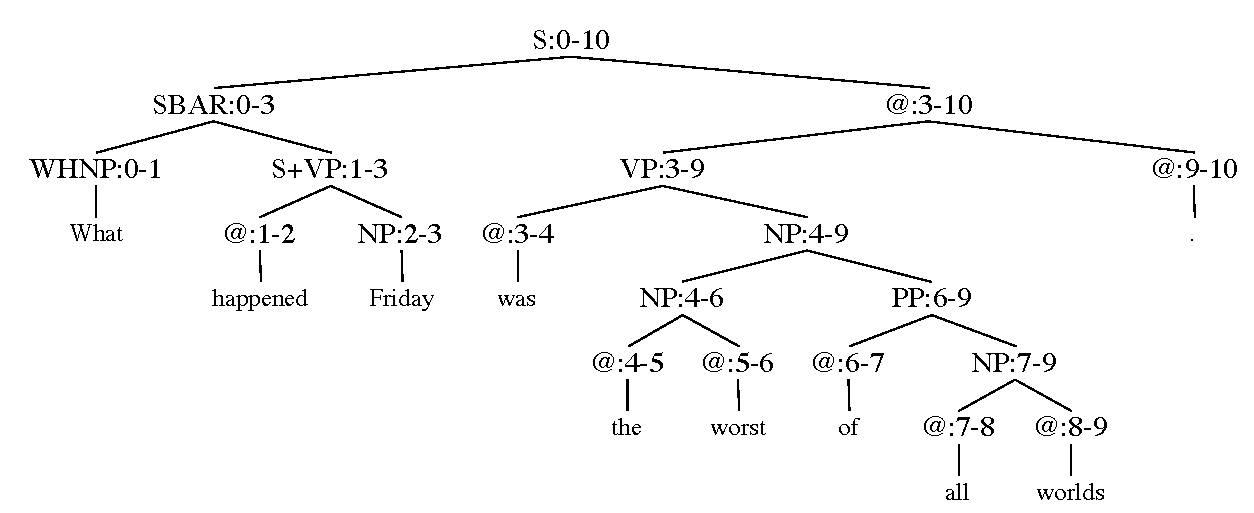
\includegraphics[width=0.9\textwidth]{../figures/trees/spans.pdf}
    \caption{In normal form with spans.}
		\label{fig:tree-cnf-spans}
	\end{subfigure}
  \caption{Converting a treebank tree (withouth part-of-speech tags).}
  \label{fig:trees}
\end{figure}

\begin{table}[]
  \footnotesize
  \begin{tabular}{l|l}
    Labeled spans & Anchored rules & \hline  \\
    (S, 0, 10)     & (S $\to$ SBAR @, 0, 3, 10) &  \\
    (SBAR, 0, 3)   & (SBAR $\to$ WHNP S+VP, 0, 1, 3) &  \\
    (VP, 1, 3)     & (S+VP $\to$ @ NP, 1, 2, 3) &  \\
    $\qquad\vdots$ & $\qquad\vdots$ &  \\
    (NP, 7, 9)     & (NP $\to$ @ @, 7, 8, 9) &  \\
  \end{tabular}
  \caption{Two conceptions of the tree in \ref{fig:tree-cnf-spans}.}
  \label{tab:spans-rules}
\end{table}

\section{Neural networks}
Introduce all the neural networks.
\begin{itemize}
  \item Feedfoward, RNN, LSTM etc.
  \item We consider these as abstractions denoting certain parametrized functions. A Feedforward network is a function that a vector $\mathbf{x}$ produces an output vector
  \begin{equation*}
    \textsc{Feedforward}_{\theta}( \mathbf{x} ) = \mathbf{y}.
  \end{equation*}
  An $\textsc{RNN}$ is function parametrized by $\theta$ that takes a sequence of vectors $\mathbf{x} = \[ \mathbf{x}_1, \dots, \mathbf{x}_n \]$  and produces a series of output vectors
  \begin{equation*}
    \textsc{rnn}_{\theta}( \mathbf{x} ) = \[ \mathbf{y}_1, \dots, \mathbf{y}_n \].
  \end{equation*}
  An $\textsc{lstm}$ is a particular way to construct the $\textsc{RNN}$ function.
  \item Maybe, maybe write down the equations for the Feedforward and the LSTM.
  \item (Minibatch) SGD optimization.
\end{itemize}

\section{Language models}
\begin{itemize}
  \item Briefly mention some typical approaches for langugage modelling: count based n-gram with smoothing \citep{Goodman+1996,Kneser+1995}, neural n-gram \citep{Bengio+2003} and recurrent neural network \citep{Mikolov+2010}. Also mention some (early) syntactic approaches: count-based \citep{Chelba2000,Klein:2012:treelets}, neural \citep{Emami+2005}, and top-down parsing related \citep{Roark2001}.
  \item Explain the metric perplexity.
  \item Briefly mentions some typical datasets and some benchmarks (dataset, perplexity, number of parameters, training time).
  \item Mention some downsides of the perplexity metric: conflating different sources of succes in next-word prediction (simple collocations, semantics, syntax).
  \item Note that there exists some alternatives to perplexity: adversarial evaluation \citep{Smith2012:adversarial}, subject-verb agreement \citep{Linzen+2016:LSTM-syntax} and grammatical acceptability judgments \citep{Linzen+2018:targeted}.
\end{itemize}

\section{Multitask learning}
\begin{itemize}
  \item Give formal description of multitask learning.
  \item In our case of language modelling with syntactic side-objective, the learning objective is to maximize
  \begin{equation*}
    \mathcal{L}(\theta, \lambda, \eta) = \sum_{ (\mathbf{x}, \mathbf{y}) \in \mathcal{D} }\log p_{\theta, \lambda}(\mathbf{x}) + \log q_{\theta,\eta}(\mathbf{y} | \mathbf{x})
  \end{equation*}
  with respect to the parameters $\theta$, $\lambda$ and $\eta$, where $p$ is our model of interest, optimized for the main objective, and $q$ is our model optimized for the side objective, which we discard after optimization.
  \item The key point of multitask learning is that the the two models $p$ and $q$ share the set of parameters $\theta$. This means that $\theta$ will be optimized to fit both objectives well.
  \item The parameters in $\lambda$ and $\eta$, in turn, are optimized to the each objective separately.
  \item The proportion and the nature of the parameters that belong to $\theta$ is a choice of the modeller and the objective.
  \item Name some recent examples of multitask learning in NLP: \cite{Zhang+2016:multitask,Goldberg+2016:multitask,Swayamdipta+2018:scaffold}.
\end{itemize}
